
Alimentamos una compuerta AND de tecnología TTL, integrado HD74LS08, conectando una entrada a la tensión Vcc y la otra al generador de funciones. Tambi\'en alimentamos una compuerta OR de tecnología CMOS, integrado SN74HC32N, conectando una entrada a tierra y la otra al generador de funciones. La alimentaciíon de ambos integrados es de 6V, el máximo sugerido por ambos fabricantes. Analizando la salida podemos notar que la compuerta OR devuelve un pico de tensión como ya notamos en la tecnología CMOS y la compuerta AND devuelve solo 3,5V a la salida, ambos parámetros están dentro de lo normal según las hojas de datos de cada una. Luego procedimos a conectar las compuertas de la siguiente forma:

\begin{figure}[hbtp]
\centering
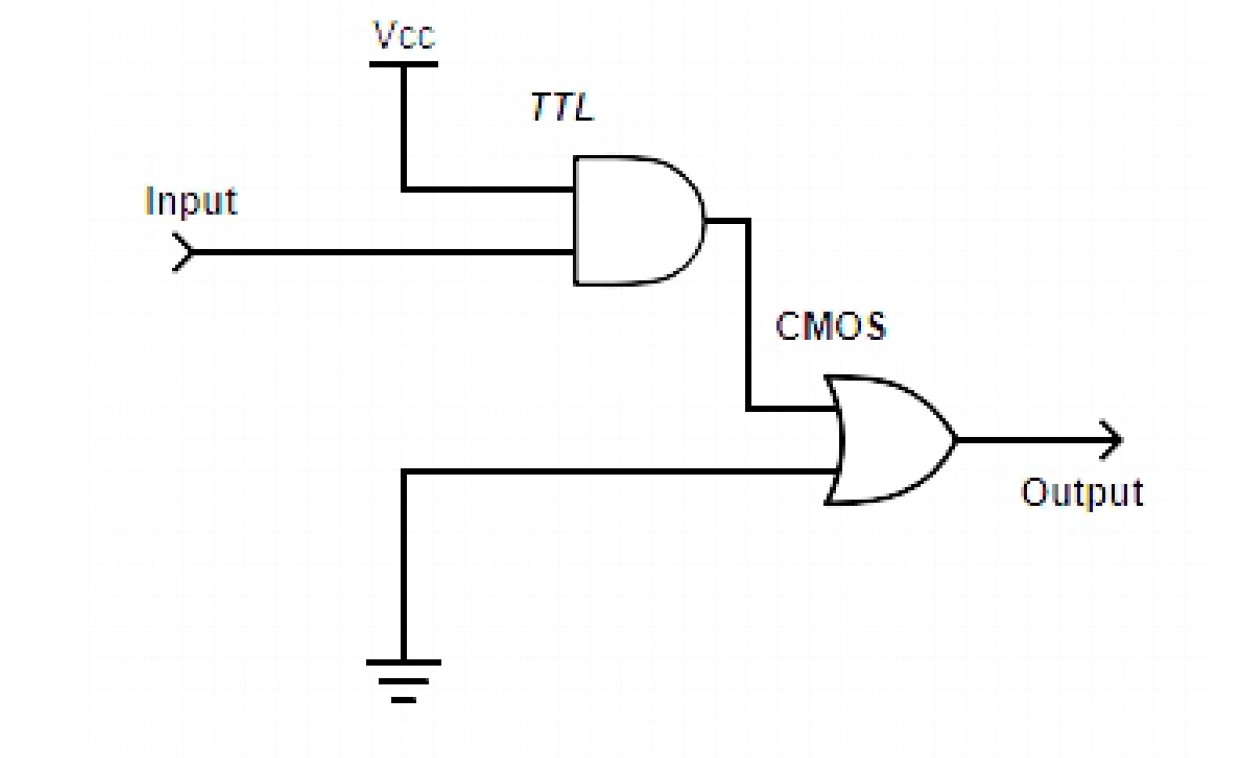
\includegraphics[width=8cm]{ejercicio5/E3_CirEj5.jpg}  
\caption{Circuito ejercicio 5}
\end{figure}


Midiendo en la salida de la OR esperaríamos que no hubiera salida o si la hubiera tuviera problemas, ya que la entrada mínima que acepta la OR es de 4,2V con la alimentación elegida y la AND otorga como ya mencionamos 3,5V. En nuestro caso el circuito lógico funcionó como si no hubiera ningún tipo de problema, creemos que esto puede deberse a que las hojas de datos otorgan datos donde el fabricante se asegura que sus componentes funcionen pero pueden haber algunos que funcionen fuera del alcance determinado por el fabricante, esto quiere decir que puede funcionar pero no esta garantizado el buen funcionamiento. En caso de haber tenido algún error hubi\'eramos optado por utilizar dos transistores para poner un pull-up que se active con la baja salida de la AND y alimente con $V_dd=5V$ la entrada de la OR como en el siguiente esquema.

\begin{figure}[hbtp]
\centering
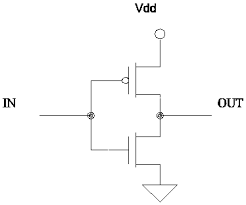
\includegraphics[width=5cm]{ejercicio5/PullUp.jpg} 
\caption{Circuito de Pull-Up}
\end{figure}

